%%%%%%%%%%%%%%%%%%%%%%%%%%%%%%%%%%%%%%%%%%%%%%%
%%% Template for lab reports used at STIMA
%%%%%%%%%%%%%%%%%%%%%%%%%%%%%%%%%%%%%%%%%%%%%%%

%%%%%%%%%%%%%%%%%%%%%%%%%%%%%% Sets the document class for the document
% Openany is added to remove the book style of starting every new chapter on an odd page (not needed for reports)
\documentclass[10pt,english, openany]{book}

%%%%%%%%%%%%%%%%%%%%%%%%%%%%%% Loading packages that alter the style
\usepackage{graphicx}
\usepackage{subcaption}
\usepackage[]{color}
\usepackage{alltt}
\usepackage[T1]{fontenc}
\usepackage[utf8]{inputenc}
\usepackage{amsfonts}
\usepackage{mathtools}
\setcounter{secnumdepth}{2}
\setcounter{tocdepth}{2}
\setlength{\parskip}{\smallskipamount}
\setlength{\parindent}{0pt}

% Set page margins
\usepackage[top=100pt,bottom=100pt,left=68pt,right=66pt]{geometry}

% Prevents LaTeX from filling out a page to the bottom
\raggedbottom

% Adding both languages
\usepackage[english, italian]{babel}

% All page numbers positioned at the bottom of the page
\usepackage{fancyhdr}
\fancyhf{} % clear all header and footers
\fancyfoot[C]{\thepage}
\renewcommand{\headrulewidth}{0pt} % remove the header rule
\pagestyle{fancy}

% Changes the style of chapter headings
%\usepackage{titlesec}
% \usepackage[Glenn]{fncychap}
% Adds table captions above the table per default
\usepackage{float}
\floatstyle{plaintop}
\restylefloat{table}

% Adds space between caption and table
\usepackage[tableposition=top]{caption}

% Adds hyperlinks to references and ToC
\usepackage{cite}
\usepackage{hyperref}
\hypersetup{hidelinks,linkcolor = black} % Changes the link color to black and hides the hideous red border that usually is created

% If multiple images are to be added, a folder (path) with all the images can be added here 
\graphicspath{ {Figures/} }

% Algorithms
\usepackage[ruled,vlined]{algorithm2e}

% Definitions
\usepackage{bm}
\usepackage{amsmath}
\newcommand{\myM}[1]{\bm{\mathit{#1}}} %Bold, italic, capital expression of matrices; vectors bold, italic, small
\newtheorem{definition}{Definition}
\DeclarePairedDelimiter\abs{\lvert}{\rvert}



% Separates the first part of the report/thesis in Roman numerals
\frontmatter
%%%%%%%%%%%%%%%%%%%%%%%%%%%%%% Starts the document
\begin{document}

%%% Selects the language to be used for the first couple of pages
\selectlanguage{english}

\author{Julian Eßer}
\title{Personal Lecture Notes \\
MITx6.832x: Underactuated Robotics \\
(Spring 2019) \\
{\Large Algorithms for Walking, Running, Swimming, Flying, and Manipulation}}

%%%%% Adds the title page
\begin{titlepage}
\maketitle
\end{titlepage}

% Adds a table of contents
\tableofcontents{}

%%%%%%%%%%%%%%%%%%%%%%%%%%%%%%%%%%%%%%%%%%%%%%%%%%%%%%%%%%%%%%%%%%%%%%%%%%%%%%%%%%%%%%%%%%%%
%%%%%%%%%%%%%%%%%%%%%%%%%%%%%%%%%%%%%%%%%%%%%%%%%%%%%%%%%%%%%%%%%%%%%%%%%%%%%%%%%%%%%%%%%%%%
%%%%% Text body starts here!
\mainmatter

\chapter{Lecture 1: Why Study Robot Dynamics?}\label{lecture1}
\section{Background / Motivation}
The \textbf{motivation} for this course is to
\begin{itemize}
\item Build great robots that can do amazing things
\item Exploit natural dynamics of robots, not just doing dump control
\item Achieve extraordinary performance in terms of speed, efficiency, or robustness (Honda's ASIMO vs. passive dynamic walkers)
\item Controlling nonlinear systems without complete control authority
\item View computation of challenging tasks in robotics (manipulation, autonomous driving) through the lense of dynamics.
\end{itemize}
This course is all about nonlinear dynamics and control of underactuated mechanical systems, with an emphasis on computational methods. Especially it covers the \textbf{topics}
\begin{itemize}
\item Nonlinear dynamics
\item Applied optimal and robust control
\item Motion planning
\item Examples from biology and applications to legged locomotion, compliant manipulation, underwater robots, and flying machines
\end{itemize}

\section{Definitions}
Nonlinear differential equations typically take the form
$$ \dot{x} = f(x,u) $$
where $f$ is a vector valued function, $x$ is the state vector and $u$ is the vector of control input and $\dot{x}=\frac{dx}{dt}$ is the time derivative.
Mechanical Systems are described by second order differential equations. When the state vector is defined as 
$$x=\begin{bmatrix}q \\ \dot{q}\end{bmatrix},$$ 
where the system dynamics can be described as
$$\ddot{q}=f(q,\dot{q}, u).$$
Since mechanical systems are \textit{control affine}, this specializes to
$$ \ddot{q}=f_{1}(q,\dot{q})+f_{2}(q,\dot{q})u.$$
A system of this form is called \textit{underactuated} if $rank[f_{2}]<=n$. 
Other causes of underactuated include
\begin{itemize}
\item Input saturation (e.g. torque limits)
\item State constraints (e.g. joint limits)
\item Model uncertainty / state estimation
\end{itemize}
 
\section{Manipulator Equations}
The equations of motion for simple systems, e.g. a double pendulum, are quite simple to derive. Results, e.g. obtained from an Lagrangian calculation approach, can be expressed in the form of the standard "manipulator equations":
$$M(q)\ddot{q}+C(q,\dot{q})\ddot{q}=\tau_{g}(q)+Bu$$ 
where $M$ is the Inertia matrix, $C$ is the matrix of Coriolis terms $\tau_{g}$ covers gravitational torques, $B$ maps inputs to generalized force and u is the control input (either force or torque).

The acceleration then is expressed as
\begin{equation}\label{eq:eom_dbl_pendl}
\ddot{q}=M^{-1}(q)[\tau_{g}(q)+Bu-C(q,\dot{q})\dot{q}].
\end{equation}
With equation \ref{eq:eom_dbl_pendl}, the dynamics of the systems and accordingly the functions $f_{1}$ and $f_{2}$ are fully defined.

For simulating the dynamics of a robot, it is sufficient to provide the  kinematics in form of a \textit{URDF file}, pass it to an forward Dynamics solver and you get the resulting acceleration and its integrations.

\section{Plan for the Course}

\begin{figure}[h!]
\begin{center}
  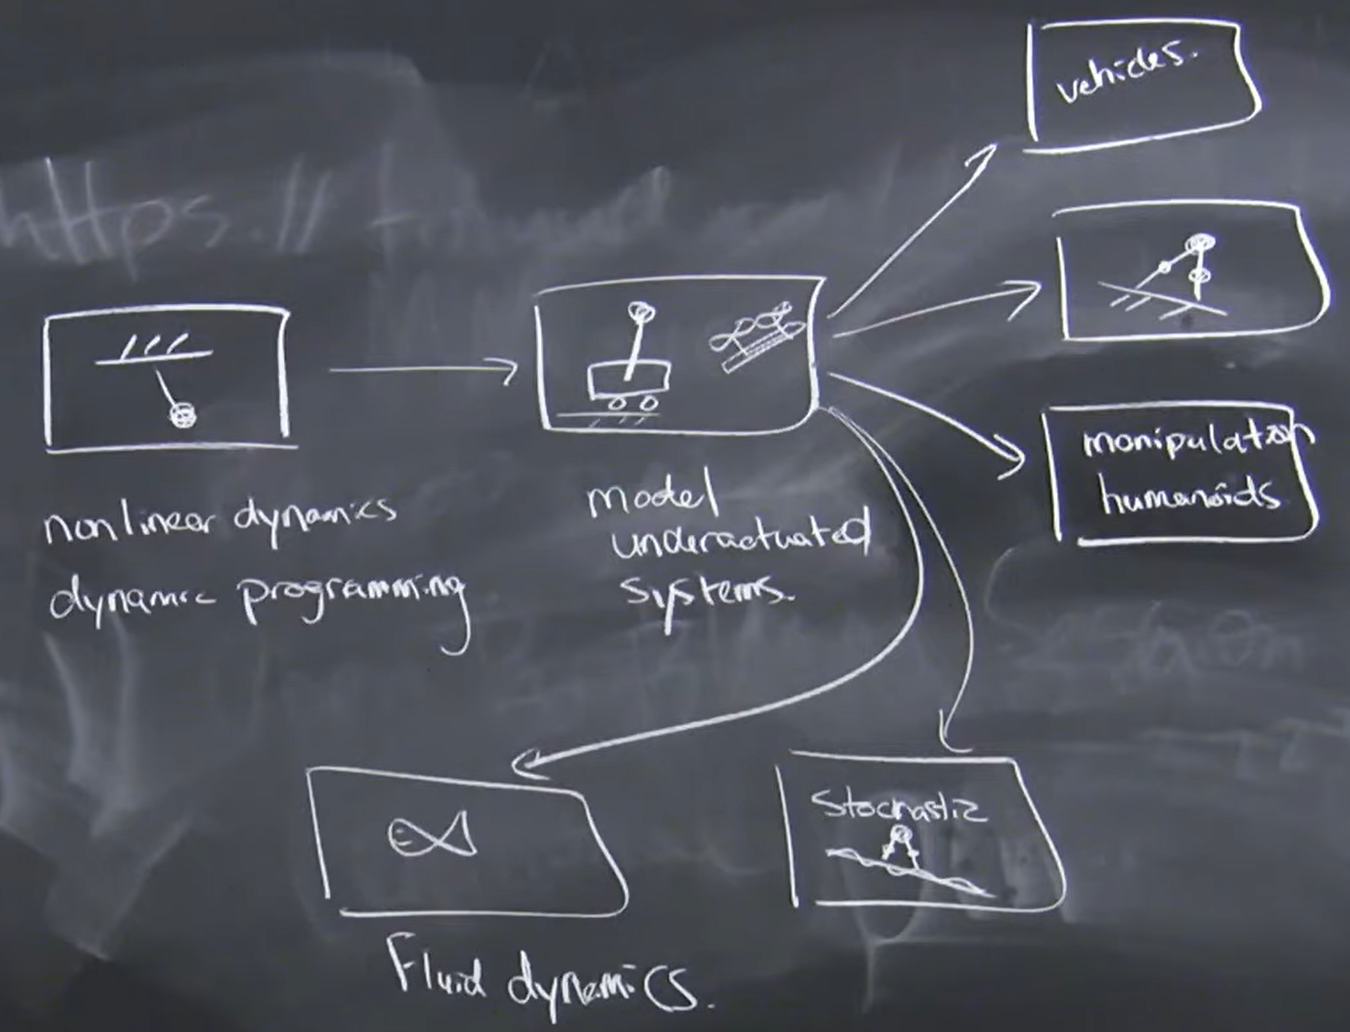
\includegraphics[width=1\textwidth]{Figures/courseOverview.png}
  \caption{Course overview: Basics first, then simple systems and then various advanced systems.}
  \label{fig:overview}
\end{center}
\end{figure}
\chapter{Lecture 2: Nonlinear Dynamics}\label{lecture2}
\section{The Simple Pendulum}
Even the most simple dynamical systems, e.g. the simple pendulum, can not be solved in a closed form. This is due to the nonlinear characteristics of the underlaying differential equations. But actually you don't have to in order to describe and analyse fundamental dynamical characteristics. 

But what we really care about is the long-term behaviour of the sytem. For low dimensional systems, two central tools are available in order to analyse the systems behaviour: 
\begin{itemize}
\item Linearization
\item Graphical Analysis
\end{itemize}
 
The equations of motion of the simple pendulum can be derived with the Langrangian as:
$$ ml^2 \ddot\theta(t) + mgl\sin{\theta(t)} = Q $$ 
Considering the generalized force $Q$ as combination of damping and a control torque input
$$ Q = -b\dot\theta(t) +u(t).$$
For the case of a constant torque this yields
$$ ml^2 \ddot\theta + b\dot\theta + mgl \sin\theta = u_0.$$

\section{Graphical Analysis}
\subsection{Fixed Points}
The central goal of control is to meaninfully shift the vector field via sophisticated control input of a system in order to change its dynamics.  
So called \textit{phase plots} are useful for visualizing this vector field of two-dimensional systems.  In case of the state vector $x= \begin{bmatrix} \theta \\ \dot{\theta} \end{bmatrix}$ this means $\dot{\theta}$ over $\theta$.

\begin{definition}
A point the system will remain forever without applying external forces is called a fixed point or a steady state respectively.
\end{definition}
The position of fixed points, e.g. stable positions of the pendulum, strongly depend on the parameter of the system (damping, input torque etc.). 

\subsection{Definitions of Stability}
There are existing different types of stability in order to describe the behaviour next a fixed point $x^{\star}$. The fixed point can be 
\begin{itemize}
\item \textit{Stable} in the sense of Lyapunov (i.e. will remain within certain radius)
\item \textit{Asymptotically stable} (i.e. for $t->\infty$ reaches certain point)
\item \textit{Exponentially stable} (reaches certain point at defined rate).
\end{itemize}

\chapter{Lecture 3/4: Dynamic Programming}\label{lecture3}
\section{Control as Optimization}
\begin{itemize}
\item The big idea is to formulate control design as an optimization problem.
\item Given a trajectory $x(.),u(.)$ we want to assign a score (scalar) to decribe the performance.
\item Additionally we can set constraints in order to exclude trajectories that exceed certain limits (e.g. control limit $\abs{u(t)}<=1$).
\item The goal is to find a control policy $u=\Pi(t,x)$ that optimizes that score!
\item When solving optimal control problems, one most often needs numerical approximation.
\end{itemize}
The strengths of Optimal Control are that it
\begin{itemize}
\item is a very general approach; it can be applied to fully/underactuated, linear/nonlinear systems,
\item contains an very intuitive approach by describing just the goal and some constraints 
\item works very well with numerical approximation.

\end{itemize}
 
 
\section{Example: Double Integrator}\begin{itemize}
\item Very simple example that can be solved without numerical approximation.
\item Consists of "brick of ice" on a flat floor
\item Goal: Go to origin as fast as possible
\end{itemize}
Easiest case: Formulate optimal control as "Bang-Bang". Accelerate (full throttle) then slam on the brakes.


\section{DDP: Discrete Time Space - Optimal Control as Graph Search}
For systems with a finite, discrete set of states and a finite, discrete set of actions, dynamic programming also represents a set of very efficient numerical algorithms which can compute optimal feedback controllers.

Cost function
$$one-step cost: g(s,a)$$
$$total cost: \sum_{n=0}^{\infty} $$
Key idea: Additive cost 
$$\int_0^T \ell(x(t),u(t)) dt,$$
There are existing numerous possibilities on how to design the cost function:
\begin{itemize}
\item Min-time: $g(s,a) = 1 "if" s~=s_{goal}; 0 if otherwise$
\item Quadratic cost: $g(x,u)=x^{T}x+u^{T}u$
\end{itemize}
There are many algorithms for finding (or approximating) the optimal path from a start to a goal on directed graphs. In dynamic programming, the key insight is that we can find the shortest path from every node by solving recursively for the optimal cost-to-go (the cost that will be accumulated when running the optimal controller) from every node to the goal.
Recursive form of the optimal control problem:
\begin{equation} \hat{J}^*(s_i) \Leftarrow \min_{a \in A} \left[ \ell(s_i,a) +
    \hat{J}^*\left({f(s_i,a)}\right) \right]
    \end{equation}
If we know the optimal cost-to-go, then it's easy to extract the optimal policy:
\begin{equation} \pi^{*}(s_i) = argmin_a
    \left[ \ell(s_i,a) + J^*\left( f(s_i,a) \right) \right].
\end{equation}

Limitations:
\begin{itemize}
\item Accuracy for continuous systems (discretisation error)
\item Scaling (curse of dimensionality)
\item Assumes full state information: Absolutely not necessary to know everything
\end{itemize}


\section{DDP: Continuous Time Space}
\subsection{The Hamilton-Jacobi-Bellman Equation}
An analogous set of conditions can be found in the continuous time space. For a system
$$ \dot{x}=f(x,u)$$
and an infinite-horizon additive cost
$$\int_0^\infty l(x,u)dt $$
we have
$$0=min_u \begin{bmatrix}
l(x,u)+\dfrac{\delta J^*}{\delta x}f(x,u)
\end{bmatrix}$$
$$\Pi^\star=argmin_u\begin{bmatrix}
l(x,u)+\dfrac{\delta J^*}{\delta x}f(x,u)
\end{bmatrix}$$








\chapter{Lecture 5-7: Acrobots, Cart-poles, and Quadrotors}
\section{Introduction}
So far we have covered the following topics:
\begin{itemize}
\item Manipulator Equations
\item Feedback Linearization
\item Optimal Control
\item Value Iteration (Algorithm for DDP in discrete time)
\end{itemize}
After introducing basics of "classic" non-linear control, we started thinking about control as optimization.

In this chapter the most simple standard models for underactuated robots are introduced. These low-dimensional systems are supposed to capture the essence of the problem without all the real-world complexity of advanced systems. 

\section{System Dynamics: Manipulator Equations}
The Acrobot is a simple underactuated system since it has two DoF. But, in comparison to the double pendulum, it only has one actuator at the elbow so that 
$\myM{B}=\begin{bmatrix} 0 & 1 \end{bmatrix}^T $.
Manipulator Equations: 
\begin{equation*}
\myM{M}(\myM{q})\myM{\ddot{q}}+\myM{C}(\myM{q,\dot{q}})\myM{\dot{q}}=\tau_g(\myM{q})+\myM{Bu}.
\end{equation*}
The goal is to swing-up and balance while satisfying some torque limits. One possible approach to solve this problem is using \textit{value iteration}. But the grids would have to be very fine, in order to get a good solution. There are better tools to solve this problem: LQR!


\section{Balancing for Acrobot and Cart-Pole}
For both the Acrobot and the Cart-Pole systems, we will begin by designing a linear controller which can balance the system when it begins in the vicinity of the unstable fixed point. To accomplish this, we will linearize the nonlinear equations about the fixed point, examine the controllability of this linear system, then using linear quadratic regulator (LQR) theory to design our feedback controller.

What we'll do to accomplish the balancing: 
\begin{enumerate}
\item Linearizing the manipulator equations
\item Check controllability of linear systems
\item Use LQR to design a feedback controller
\end{enumerate}
\subsection{Recap: LQR}
We have a linear time-invariant system in state-space form
\begin{equation*} 
\myM{\dot{x}}=\myM{Ax}+\myM{Bu},
\end{equation*}
the cost function is 
\begin{equation*} 
J = \int_0^{\infty}[\myM{x}^T\myM{Qx}+\myM{u}	^T\myM{Ru}]dt,
\end{equation*}
and the goal is to find the optimal cost-to-go function $J^\star(\myM{x})$ which satisfies the Hamilton-Jacobi-Bellman equation.
This yields 
\begin{equation*} 
J^\star(\myM{x}) = \myM{x}^T\myM{Sx}
\end{equation*}
and the optimal control policy 
\begin{equation*} 
\myM{u}^\star=\myM{Kx}.
\end{equation*}
In the end, this means you get the control policy and the cost-to-go function by
\begin{equation*} 
\myM{K,S}=LinearQuadraticRegulator(\myM{A}, \myM{B}, \myM{Q}, \myM{R}).
\end{equation*}
So you set $\myM{A}, \myM{B}$ from linearization and choose $\myM{Q}, \myM{R}$ and receive an optimal controller.

\subsection{Linearization of Nonlinear Systems}
\textbf{Problem:} Our systems are non-linear! How shall we apply Linear-Quadratic Control?!

\textbf{Solution:} We linearize our system around a specific fixed point.

But we need to be aware that our linearization only is valid within a certain area around this point. If you go to far away from it, the non-linearity overwhelms your solution. 

One Optimal Control Algorithm therefore is to combine multiple LQR Controllers that treat all relevant fixed points in order to handle the relevant workspace. 

\section{Throwback: Hand-Designed Control}
\begin{itemize}
\item Optimal control is a powerful framework for solving control problems via optimization.
\item Solving OC problems for non-linear systems is hard!
\item Sometimes we would be happy to just have any controller (And sometimes they turn out to be even better).
\item But how can we proof this "hand-designed" are any good? 
\end{itemize}

\section{Partial Feedback Linearization (Acrobot,Cart-pole)}
Although we cannot always simplify the full dynamics of the system, it is still possible to linearize a portion of the system dynamics. The technique is called partial feedback linearization.
\begin{itemize}
\item \textit{Collocated} PFL: A controller which linearizes the dynamics of the \textit{actuated} joints
\item \textit{Non-Collocated} PFL: A controller which linearizes the dynamics of the \textit{unactuated} joints
\end{itemize}
One of the most important lessons from partial feedback linearization, is the idea that if you have m actuators, then you basically get to control exactly m quantities of your system.

-> We proof that they are stable. 

\section{Swing-Up Control: Energy Shaping (Acrobot,Cart-pole)}
If we seek to design a nonlinear feedback control policy which drives the simple pendulum from any initial condition to the unstable fixed point, a very reasonable strategy would be to use actuation to regulate the energy of the pendulum to place it on this homoclinic orbit, then allow the system dynamics to carry us to the unstable fixed point.

This idea turns out to be a bit more general than just for the simple pendulum. As we will see, we can use similar concepts of `energy shaping' to produce swing-up controllers for the acrobot and cart-pole systems. It's important to note that it only takes one actuator to change the total energy of a system.

The basic Idea for the swing-up control is to
\begin{enumerate}
\item Use collocated PFL to simplify the dynamics
\item Use energy shaping to regulate the pendulum to its homoclinic orbit
\item Add a few terms to make sure that the cart stays near the origin
\end{enumerate}


\section{Differential Flatness (Quadrotors)}
The task we'll consider for quadrotors is trajectory optimization:

How can you find a feasible trajectory through state space for the quadrotor, even if there are obstacles to avoid that are only known at runtime? 

Trajectory design, and especially trajectory optimization, is a big idea that we will explore more thoroughly later in the text. But there is one idea that I would like to present here, because in addition to being a very satisfying solution for quadrotors, it is philosophically quite close to the idea of partial feedback linearization. That idea is called differential flatness.

\begin{itemize}
\item Similar idea as PFL: Given a trajectory of m (number of actuators) coordinates. 
\item Then, the control input and all left states can be guessed
\item Condition: Trajectory needs to be four-times differentiable
\end{itemize}

2D-Quadrotor Example (m=2): Given x,y of trajectory, guess resulting jaw and control input.

3D-Quadrotor Example (m=4): Given x,y,z,jaw guess roll, pitch and control for all motors.


\chapter{Lecture 8/9: Lyapunov Analysis}
Optimal control provides a powerful framework for formulating control problems using the language of optimization. But solving optimal control problems for nonlinear systems is hard! In many cases, we don't really care about finding the optimal controller, but would be satisfied with any controller that is guaranteed to accomplish the specified task. In many cases, we still formulate these problems using computational tools from optimization, and in this chapter we'll learn about tools that can provide guaranteed control solutions for systems that are beyond the complexity for which we can find the optimal feedback.


\section{Lyapunov Functions}
\subsection{Optimization Crash Course}
\begin{itemize}
\item Goal: Find $x_{min}$ for an objective (cost) function considering a set of (in/equality-) constraints
\item Popular objective functions:
\begin{itemize}
\item Convex quadratic cost (least squares)
\item Linear cost
\end{itemize}
\item Convex optimization builds on convex cost functions or a convex set
\end{itemize}

\subsection{Introduction}
Lyapunov functions generalize the notion of an energy function to more general systems, which might not be stable in the sense of some mechanical energy. If I can find any positive function, call it$V(\myM{x})$, that gets smaller over time as the system evolves, then I can potentially use $V$ to make a statement about the long-term behavior of the system. $V$is called a Lyapunov function. 


\section{Lyapunov Analysis with Convex Optimization}
In this section, we'll look at some computational approaches to verifying the Lyapunov conditions, and even to searching for (the coefficients of) the Lyapunov functions themselves.
\subsection{Lyapunov Analysis for Linear Systems}
Imagine you have a linear system
$\myM{\dot{x}}=\myM{Ax},$
and can find a Lyapunov function
$$V(\myM{x})=\myM{x}^T\myM{Px}, \myM{P}=\myM{P}^T>0,$$
which also satisfies
$$\myM{\dot{V}(x)}=\myM{x}^T\myM{PAx}+\myM{x}^T\myM{A}^TPx<0.$$
Then the origin is globally asymptotically stable.

\subsection{Lyapunov Analysis as a Semi-definite Program (SDP)}
Lyapunov analysis for linear systems has an extremely important connection to convex optimization. In particular, we could have also formulated the Lyapunov conditions for linear systems above using semi-definite programming (SDP). Semidefinite programming is a subset of convex optimization -- an extremely important class of problems for which we can produce efficient algorithms that are guaranteed find the global optima solution 
\subsection{Sums-of-squares Optimization}
It turns out that in the same way that we can use SDP to search over the positive quadratic equations, we can generalize this to search over the positive polynomial equations.


\section{Lyapunov Analysis for Estimating Regions of Attraction}
There is another very important connection between Lyapunov functions and the concept of an invariant set: any sub-level set of a Lyapunov function is also an invariant set. This gives us the ability to use sub-level sets of a Lyapunov function as approximations of the region of attraction for nonlinear systems.

Now we have arrived at the tool that I believe can be a work-horse for many serious robotics applications. Most of our robots are not actually globally stable (that's not because they are robots -- if you push me hard enough, I will fall down, too), which means that understanding the regions where a particular controller can be guaranteed to work can be of critical importance.

Sums-of-squares optimization effectively gives us an oracle which we can ask: is this polynomial positive for all x? To use this for regional analysis, we have to figure out how to modify our questions to the oracle so that the oracle will say "yes" or "no" when we ask if a function is positive over a certain region which is a subset of R. That trick is called the S-procedure. It is closely related to the Lagrange multipliers from constrained optimization, and has deep connections to "Positivstellensatz" from algebraic geometry.


\chapter{Lecture 10: Trajectory Optimization}
\section{Recap: What Did We Cover so Far?}
The\textbf{ overall goal} is to specify complex behaviors with simple objective functions, letting the dynamics and constraints on the system shape the resulting feedback controller.

But the computational tools that we've provided so far have been \textbf{limited} in some important ways:
\begin{itemize}
\item \textbf{Dynamic programming} involves putting a mesh over the state space 

-> Stuck in low-dimensional systems.
\item \textbf{LQR} + \textbf{Linearization} around an operating point; applicable to high-dimensional systems 

-> Linearization only valid for a certain region of the state space
\item \textbf{Lyapunov Analysis via SDP/SOS} softens the requirements by not searching for the optimal controller, but only searching for stability. It does so for non-linear systems and all $\myM{x}$ (whole state-space).

-> No controller actually synthesised + somehow limited to simple Lyapunov functions (quadratic, polynomials etc) which might limit the control design  
\end{itemize}
But we have not yet provided any real computational tools for approximate optimal control that work for high-dimensional systems beyond the linearization around a goal. That is precisely the goal for this chapter.

\textbf{Q:} How can we handle complex systems?

\textbf{A:} We ask not for all states (like in Lyapunov Analysis), instead only the relevant ones!
\begin{itemize}
\item For the beginning: Consider only one single initial condition!
\item Maybe some $x_0$ in the neighbourhood are also good
\item Represent the solution as a trajectory,  $\myM{x}(t), \myM{u}(t)$, typically defined over a finite interval (instaed of feedback control function)
\item \textbf{This means:} 
\begin{enumerate}
\item We define only a single trajectory $\myM{u}(t)$, 
\item Search for optimal states $\myM{x}$ and control inputs $\myM{u}$,
\item To follow this trajectory as good as possible!
\end{enumerate}
\end{itemize}


\section{Problem Formulation}
\begin{itemize}
\item Min over a finite trajectory over time $\myM{u}(\cdot)$
\item Initial conditions $x(0)$ are fixed and known
\end{itemize}
\begin{align*}
\min_{\myM{u}(\cdot)} \quad &
\int_{t_0}^{t_f} \ell(\myM{b}(t),\myM{b}(t)) dt \\ \text{subject to} \quad &
\forall t, \dot{\myM{x}}(t)=f(\myM{x}(t),\myM{u}(t)), \\
& \myM{x}(t_0)=x_0
\end{align*}


\section{Computational Tools for Nonlinear Optimization}
Intro 
\section{Trajectory Optimization as a Nonlinear Program}
As written above, the optimization above is an optimization over continuous trajectories. In order to formulate this as a numerical optimization, we must parameterize it with a finite set of numbers. 

Different approaches on how to do this, are:
\begin{itemize}
\item Idea 1). \textbf{Direct Transcription}: Fix breakpoints at even intervals $dt$ and use Euler integration. Decision variables are $x,n$ 
\item Idea 2.) \textbf{Direct Shooting Methods} - Idea: Destrict decision variables to only $u$ and and compute $x$ ourselves by knowing $x_0$ and $u(\cdot)$ via the simple forward dynamics
$$x[t=0] = x_0$$
$$x[1]=Ax_0+Bu[0]$$
$$x[2]=A\cdot(x[1]=Ax_0+Bu[0])+Bu[0]$$
$$...$$
\item Idea 3.) \textbf{Direct Collocation:} Assume first-order polynomial for $\myM{u}(t)$ and cubic polynomial $\myM{x}(t)$.
\end{itemize}


\section{Pontryagins's Minimum Principle}


\section{Trajectory Stabilization: Local Trajectory Feedback Design}
What we want is to move robots in the real world. Therefore it is not useful to have only one exact trajectory, but we need to allow the robot to move in a \textbf{band around our target trajectory}. 

\textbf{Idea}: Locally linearize around our points from the trajectory, so that we can apply tools from linear control again.

\subsection{Linear Model-predictive Control}
Locally stabilizes a \textbf{constrained} system.
\subsection{Time-varying LQR}
Locally stabilizes $\myM{x}_0(t), \myM{u}_0(t)$

\section{Iterative LQR}



  



\chapter{Lecture 12/13: Simple Models of Walking and Running}
In this chapter we'll introduce some of the simple models of walking and robots, the control problems that result, and a very brief summary of some of the control solutions described in the literature. Compared to the robots that we have studied so far, our investigations of legged locomotion will require additional tools for thinking about limit cycle dynamics and dealing with impacts.


\section{Limit Cycles}
In many of the systems that we have studied so far, we have analyzed the stability of a fixed-point, or even an (infinite-horizon) trajectory. For walking systems the natural equivalent is to talk about the stability of periodic solutions -- a fixed "gait" is a cycle that repeats footstep after footstep. So we begin our discussion with a discussion of the stability of a cycle.
A limit cycle is an asymptotically stable or unstable periodic orbit. One of the simplest models of limit cycle behavior is the Van der Pol oscillator.
\subsection{Poincare Maps}


\section{Simple Models of Walking}
\subsection{The Rimless Wheel}
The most elementary model of passive dynamic walking, first used in the context of walking by, is the rimless wheel. This simplified system has rigid legs and only a point mass at the hip as illustrated in the figure above. To further simplify the analysis, we make the following modeling assumptions
\begin{itemize}
\item No slip
\item Collisions are inelastic and impulsive (no bouncing)
\item No double support
\end{itemize}
\subsection{The Compass Gait}
\subsection{The Kneed Walker}


\section{Simple Models of Running}
There are existing various definitions of running:
\begin{itemize}
\item Existence of an Aerial Phase
\item Exchange of Energy 
\end{itemize}
Why do we study simple models?
\begin{itemize}
\item Tractable
\item Mechanical Insights
\item Comparative Biology: Fundamental Principles?
\item As a 'Template' for Higher-DOF Robots
\end{itemize}
\subsection{The Spring-Loaded Inverted Pendulum}
\subsubsection{Assumptions}
\begin{itemize}
\item Masless leg -> command $\theta$ instantaneously
\item Perfectly \textbf{elastic} collision -> Energy is always conserved (thread to stability)
\item When the foot is on ground, we have a pin joint i.e. infinite friction (no sliding)
\end{itemize}
\subsubsection{SLIP Modeling}
The model is a point mass, $m$ , on top of a massless, springy leg with rest length of
$l_0$, and spring constant $k$. The state of the system is given by $x,y$ the position of the center of mass, and the length,$l$ , and angle $\theta$ of the leg. Like the rimless wheel, the dynamics are modeled piecewise - with one dynamics governing the flight phase, and another governing the stance phase.

Flight Phase. State variables: $\myM{x}=[x,y,\dot{x},\dot{y}]^T$. Dynamics are
$$\dot{\myM{x}}\begin{bmatrix} \dot{x} \\ \dot{y} \\ 0 \\ - g
      \end{bmatrix}.$$
      
Stance Phase. State variables: $\myM{x}=[r,\theta, \dot{r},\dot{\theta}]$. Kinematics are
$$x = \begin{bmatrix} - r \sin\theta \\ r
      \cos\theta \end{bmatrix}.$$
Energy is given by
$$T = \frac{m}{2}
      (\dot{r}^2 + r^2 \dot\theta^2 ), \quad U = mgr\cos\theta +
      \frac{k}{2}(r_0 - r)^2.$$
Putting these into Lagrange yields:
\begin{equation}
  m \ddot{r} - m r \dot\theta^2 + m g \cos\theta - k (r_0 -r) = 0  
\end{equation}
\begin{equation}
m r^2 \ddot{\theta} + 2mr\dot{r}\dot\theta - mgr \sin\theta = 0
\end{equation}
\subsubsection{SLIP Control}
Choose $\theta_{touchdown}$ during aerial phase. 

Goal: Design controller $u[n]=\Pi(y[n])$ to stabilize $y^d$.
\begin{itemize}
\item Idea 1: find $u\star$ st. $y^\star=P(y^d,u^\star)$. 

\textbf{Linearize} P around $(y^d, u^p)$ + do (discrete time) \textbf{LQR}.

Results in an exponential convergence to the fixed point. 
\item Idea 2: Deadbeat Control.

If P is invertible,
$$u[n]=P^{-1}(y^d,y[n])$$
If exists, results in an convergence to the fixed-point via one timestep.
\end{itemize}

\subsection{Continuous Control: The Planar Monopod Hopper}
\begin{itemize}
\item Hopping Height (push at toe-off)
\item Foot Touchdown to regulate speed
\item Stabilize attitude during stance
\end{itemize}

\section{A Simple Model That Can Walk and Run}








\chapter{Lecture 14/15: Planning and Control Through Contact}
So far we've discovered the following tools:
\begin{itemize}
\item Fixed Points / Local Stability
\item Local Stabilization (e.g. LQR)
\item Lyapunov Analysis
\item Trajectory Optimization
\end{itemize}
These tools work out for "smooth" systems where the equations of motion are described by a function $\dot{\myM{x}}=f(\myM{x},\myM{u})$ which is smooth everywhere. But our discussion of the simple models of legged robots illustrated that the dynamics of making and breaking contact with the world are more complex -- these are often modeled as \textbf{hybrid dynamics} with \textbf{impact} discontinuities at the collision event \textbf{and constrained dynamics} during contact (with either soft or hard constraints).

The goal of this chapter is to extend our computational tools into this richer class of models. Many of our core tools still work: trajectory optimization, Lyapunov analysis (e.g. with sums-of-squares), and LQR all have natural equivalents. 

\section{Modeling Contacts}
We can model the robot in \textbf{floating-base coordinates} -- we add a fictitious six degree-of-freedom "floating-base" joint connecting some part of the robot to the world (in planar models, we use just three degrees-of-freedom. We can derive the equations of motion for the floating-base robot once, without considering contact, then add the additional constraints that come from being in contact as contact forces which get applied to the bodies. The resulting manipulator equations take the form
$$\myM{M}(\myM{q})\ddot{\myM{q}}+\myM{C}(\myM{q,\dot{q}})\dot{\myM{q}}=\tau_g(\myM{q})+\myM{Bu}+\sum_i\myM{J}_i^T(\myM{q})\lambda_i,$$
where $\lambda_i$ are the contact forces and $J_i$ are the contact Jacobians. 
Conveniently, if the guard function in our contact equations is the signed distance from contact, $\phi_i(\myM{q})$, then this Jacobian is simply $\myM{J}_i(\myM{q})=\dfrac{\partial\phi_i}{\partial\myM{q}}$.

\section{Trajectory Optimization}
\section{Randomized Motion Planning}
\section{Stabilizing a Trajectory or Limit Cycle}



\chapter{Lecture 16: Highly-Articulated Legged Robots}
We've adressed many of the simple walking models in previous chapters. It turns out that there at some point by adding more and more DoFs, the OC gets easier again. This is the case if we can nearly arbitrarily place our foots wherever we want.

For Humanoids new tools come along, which will be covered within this chapter. 


\section{Center of Mass Dynamics}
When we think of a robots base with massless legs, it's actually comparable to a Hovercraft flying around in space. We have to add some constraints: 
\begin{itemize}
\item Constraining the input torque
\item The thrusters are movable
\item Thrusters are off when they are moving
\item Velocity is limited
\item Thrusters only can be turned on in certain regions
\end{itemize} 
Therefore the analogy makes sense: Masslegs legs are comparable to little thrusters.

One strategy that many humanoids use is to
\begin{itemize}
\item Keep the center of mass at a constant height and then
\item Minimize the angular momentum about the center of mass
\end{itemize}
This is a totally different view then before, since it is on a much higher level. And it turns out it is even meaningful if we consider legs that do have masses. 

Then, if we are really able to stabilize the CoM and total angle of momentum, the problem formulation gets a way easier, since
\begin{itemize}
\item we can effectively neglect the impulse dynamics, since the velocity of a foot touching the ground will be nearly zero!
\item The EoMs are linear!
\end{itemize}
 

\section{The Special Case of Flat Terrain}
This is the environment where most humanoids start walking. In this situation the constraints on the center of mass dynamics can be summarized very efficiently.

Let us define the "center of pressure" (CoP) as the point on the ground where 
$$x_{cop} = \frac{\sum_i p_{i,x} F_{i,z}}{\sum_i
    F_{i,z}},$$
and since all $p_{i,z}$ are equal on flat terrain, $z_{cop}$ is just the height of the terrain. It turns out that the center of pressure is a "zero-moment point" (ZMP) -- a property that we will demonstrate below -- and moment-balance equation gives us a very important relationship between the location of the CoP and the dynamics of the CoM: 
$$(m\ddot{z} + mg)
    (x_{cop} - x) = (z_{cop} - z) m\ddot{x} - I\ddot\theta.$$
    
If we use the strategy proposed above for ignoring collision dynamics, $\ddot{z}=\ddot{\theta}=0$, then we have $z-z{cop}$ is a constant height $h$, and the result is the famous "ZMP equations": 
$$\ddot{x} = -\frac{g}{h}
    (x_{cop}-x).$$
So the location of the center of pressure completely determines the acceleration of the center of mass, and vice versa!


\section{Zero Moment Point (ZMP) Planning}
For rigid body systems I can always summarize the contributions from many external forces as a single wrench (force and torque) on the object. For walking robots, it is this point on the ground from which the external wrench can be described by a single force vector (and no moment) that is the famous "zero-moment point".

On the spatial case of flat terrain $x{cop}$ is a ZMP!

And we can use this simple relation to derive more complicated plans for the robot. State of the art is a three step walking plan/control:
\begin{enumerate}
\item Footstep planning (Decide where to place the foots)
\item Plan COM \& COP
\item Fill in the details ($q,\dot{q}$)
\end{enumerate}  
Some remarks/insights on this algorithm:
\begin{itemize}
\item CoP always needs to be within the support polygon
\item It also works for pure position control -> Based on the footplan you derive an exact CoP trajectory that is a set of straight lines and follow it - Timing is important
\item From a control perspective, walking fast is easier than walking slowly. This is because the CoM is more straight while walking slowly the CoM trajectory is closer to the Footsteps (i.e. more shifting)
\item Earlier: people hardcoded the CoP trajectory
\item Now: Since the equations appeared are linear, we can use linear optimal control to solve for the CoP/CoM trajectory! E.g. you can optimize the robots behaviour to follow a desired CoM trajectory as close as possible while reducing the amount of energy
\end{itemize}


\section{Footstep-Planning and Push Recovery}
There was a time when footstep-planning where thought of an AI problem, but we can do better now. Some methods for coming up with footstep plans include
\begin{itemize}
\item Sampling-based
\item Nonlinear-trajectory optimization
\item Mixed-integer convex optimization
\end{itemize}
The special thing about footstep plans is that they use very simple models (if any models at all). Especially using
\begin{itemize}
\item Simplified kinematics and 
\item Almost no dynamics (e.g. inverted-pendulum models)
\end{itemize}
during the general planning. 

\textbf{Clarification: Static vs. Dynamic Walking:}
\begin{itemize}
\item With quasi static walking, the CoM at each point in time has to be within the support polygon of the robot (low efficiency, low $v_{max}$)
\item Dynamic Walking in contrast is not constrained as hard in this way. It allows for 'instable' intermediate phases. Nevertheless, the CoP has to be within the support polygon.  
\end{itemize}
Asimo uses static walking, ZMP is in this sense unstable but it is an desired pattern towards more efficient and faster locomotion. 


\section{Whole-Body Control}


\section{Beyond ZMP Planning}







\chapter{Lecture 17: Motion Planning as Search}
Another tool for our toolbox: Complete Planning is one of the key problems left for us to tackle. This especially means to always find an answer to the question: Is it possible for this robot to reach a specific goal or not.

Two state of the art approaches include
\begin{itemize}
\item Decompose non-convexity in problem, then search all decompositions
\item Randomized motion problem
\end{itemize}  

The \textbf{future solution} might lay somewhere in between: While the randomized algorithms are extremely powerful, it somehow feels a bit strange that we do not make (partly) use of the geometric knowledge of the environment that we have from perception.


\section{Artificial Intelligence as Search}
Def: A planner is said to be \textbf{complete}, if it is guaranteed to find a solution if one exists.

Def: A planner is said to be \textbf{globally optimal} if it finds the optimal plan.

\section{Randomized Motion Planning}
These algorithms are fairly simple, extremely powerful and became state of the art nowadays. They belong to the group of \textbf{sampling-based planners}. The RRT is one algorithm that can be applied to underactuated systems. 
\subsection{Rapidly-Exploring Random Trees (RRTs)}
The basic algorithm: 
\begin{enumerate}
\item Generate a random sample
\item Discard the ones initialized within boundaries of objects
\item Find closest point on current track
\item Extend tree towards sample point
\end{enumerate}
\subsection{RRTs for Robots with Dynamics}
It shows that RRTs even work surprisingly well for high-dimensional search spaces, i.e. robots with many DoFs. If you know the kinematics well. 


\subsection{Variations and Extensions}
Possible improvements are
\begin{itemize}
\item Better sampling distributions
\item Better distance metric
\item Better extension 
\end{itemize}


\section{Decomposition Methods}
The idea:
\begin{itemize}
\item Decompose the environment into accessible regions, i.e regions where the quadrotor should stay within
\item Search for all of these decompositions
\end{itemize}
This approach is an option, but it is an \textbf{very expensive} way for seeking towards completeness. 
\chapter{Lecture 18: Feedback Motion Planning}
\textbf{[Complete when online notes have been added!]} 

The randomized motion planning methods from the last chapter deliver impressive results. However, their application to complex robots is limited due to efficiency and robustness issues of just \textbf{random movements} with your robot in order to get to the road. 

In other words: Solely thinking about resulting \textbf{trajectories} probably wont win the game. This is especially true since complex interactions with the environment have a highly need of \textbf{providing feedback} from the done actions and consider them for the next control steps. 

\section{Probabilistic Feedback Coverage}
In order to provide robustness for complex tasks, one can think of the following approach
\begin{itemize}
\item We imagine a 'funnel' (robustness area) around our desired trajectory
\item This funnel is formed via some Lyapunov function (cubic spline)
\item A complex robots behavior (e.g. walking and then trotting) can be modeled as phases where different 'skills' are required
\item Each skill (i.e. controller), bounded by a Lyapunov function, ensures that it's last is feasible for the init of the following up skill 
\end{itemize}

\section{Drawbacks}
\begin{itemize}
\item Offline control method
\item Again, this method highly depends on the knowing the whole state space of the robot. 
\item Therefore, it also does not suit very well for complex systems
\end{itemize}
\chapter{Lecture 19: Model Systems with Stochasticity}
So far: 
$$\dot{\myM{x}}=f(\myM{x},\myM{u}).$$
Now: 
$$\dot{\myM{x}}=f(\myM{x},\myM{u},\myM{w}),$$
where $\myM{w}$ is the output of some random process. Here we only cover \textbf{process noise}, caused by:
\begin{itemize}
\item Disturbances
\item Model Uncertainty
\end{itemize}
Measurement noise will not be considered here.

Every time that we've analyzed a system to date, we've asked questions like "given x[0], what is the long-term behavior of the system? But now $x[n]$ is a random variable. The trajectories of this system do not converge, and the system does not exhibit any form of stability that we've introduced so far. 


\section{The Master Equation}
All is not lost. The \textbf{distribution} of this random variable is actually very well behaved. This is the key idea for this chapter. Let us use $p_n(x)$ to denote the probability density function over the random variable $\myM{x}$ at time $n$.

It is actually possible to write the dynamics of the probability density with the simple relation 
$$p_{n+1}(x) = \int_{-\infty}^\infty p(x|x') p_n(x') dx',$$
where $p(x|x')$ encodes the stochastic dynamics as a conditional distribution of the next state (here x) as a function of the current state (here $x'$). Dynamical systems that can be encoded in this way are known as continuous-state Markov Processes, and the governing equation above is often referred to as the "master equation" for the stochastic process.


\section{When Do We Actually Need This Kind of Modeling?}
Let's answer this question by two different kinds of disturbances that can be applied to legged locomotion: 
\begin{itemize}
\item \textbf{The robot gets kicked:} One huge impact, but the model is correct for most of the time (after recovery from push and before being kicked
\item \textbf{The robot is walking on uneven terrain:} The model of flat terrain is wrong for all the time. Here it makes sense to add stochasticity to the modeling approach.
\end{itemize}
\chapter{Lecture 20: Robust and Stochastic Control}
Goal: Obtain guarantees for constraints for a stochastic (non-deterministic) system.
\section{Discrete states and actions}
\section{Linear Quadratic Gaussian (LQG)}
\section{Linear Exponential-Quadratic Gaussian (LEQG)}
\chapter{Lecture 22/23: Reinforcement Learning}
Reinforcement learning (RL) is a \textbf{collection of algorithms} for solving the same optimal control problem that we've focused on through the text, but the real gems from the RL literature are the algorithms for (almost) \textbf{black-box optimization} of \textbf{stochastic optimal control problems}. The idea of an algorithm that only has a "black-box" interface to the optimization problem means that it can obtain (potentially noisy) samples of the optimal cost via trial and error, but does not have access to the underlying model, and does not have direct access to complete gradient information.

\begin{itemize}
\item How do we optimize? "Black-box Optimization": $\sum g(x,u)$ -> We \textit{don't} have a model, only costs
\item What do we optimize? "Stochastic OC Problems": $\min \myM{E}[(x,u)]$ with \textit{random} variables
\end{itemize}

Motivation for RL:
\begin{itemize}
\item For complex problems: When we don't have a model, or the model would be to complex for control design
\end{itemize}

Relation RL / OC:
\begin{itemize}
\item RL more general 
\item OC more efficient (RL random try/error)
\end{itemize}

Drawbacks RL
\begin{itemize}
\item Computationally extremely consumptive (try and error)
\item Manual tuning of parameters necessary
\end{itemize}

\textbf{Overall objective to define}: What to learn? 
\begin{enumerate}
\item Learn $f(x,u)$: System identification + Model-based control
\item Learn $\Pi(x)$: Policy Search -> Section \ref{sec:policy-based}
\item Learn $\hat{J}(x)$: Cost-to-go -> Section \ref{sec:value-based}
\end{enumerate}

\section{Policy-Based Methods}\label{sec:policy-based}
\subsection{The Policy Gradient "Trick"}
One of the standard approaches to policy search in RL is to estimate the gradient of the expected long-term cost with respect to the policy parameters by evaluating some number of sample trajectories, then performing (stochastic) gradient descent. Many of these so-called "policy gradient" algorithms leverage a derivation called the likelihood ratio method that was perhaps first described in [2] then popularized in the the REINFORCE algorithm [3]. It is based on what looks like a trick with logarithms to estimate the gradient

The surprise: I can find the gradient of the long-term cost by taking only the gradient of the policy... but not the gradient of the plant, nor the cost! The intuition is that one can obtain the gradient by evaluating the policy along a number of (random) trajectory roll-outs of the closed-loop system, evaluating the cost on each, then increasing the probability in the policy of taking the actions correlated with lower long-term costs.


\section{Sample Performance via the Signal-to-Noise Ratio}
The simplicity of the REINFORCE / weight perturbation updates makes it tempting to apply them to problems of arbitrary complexity. But a major concern for the algorithm is its performance - although we have shown that the update is in the direction of the true gradient on average, it may still require a prohibitive number of computations to obtain a local minima.
In this section, we will investigate the performance of the weight perturbation algorithm by investigating its signal-to-noise ratio (SNR).


\section{Value-Based Methods}\label{sec:value-based}
Key Idea: Learning value function.




\pagebreak
% Adding a bibliography if citations are used in the report
\bibliographystyle{plain}
\bibliography{literature.bib}
% Adds reference to the Bibliography in the ToC
\addcontentsline{toc}{chapter}{\bibname}

\pagebreak



\end{document}
